\documentclass[svgnames,table,,aspectratio=169]{beamer}
%\documentclass[svgnames,table,handout,aspectratio=129]{beamer}
\usepackage{hhline}
\usepackage{etoolbox}
\usepackage{tikz}
\usepackage{mathtools}
\usepackage{amssymb}
%\usepackage{/usr/lib64/R/share/texmf/Sweave}
\usepackage{polynom}
\usepackage{qrcode}


%\input{latexdefinitions}
\definecolor{georgiaRed}{RGB}{100,0,00}
\definecolor{mediumGray}{gray}{0.6}



\usetheme{Frankfurt}%
%\usetheme{Warsaw}%
%\useoutertheme{smoothbars}


%\usecolortheme{seagull}
\usecolortheme{beaver}
\logo{\includegraphics[height=.125in]{ugaLogo}}

% Note that the colour definitions are given in the latexDefinitions
% file.
\setbeamercolor{palette primary}{fg=georgiaRed,bg=white}
\setbeamercolor{palette secondary}{fg=georgiaRed,bg=white}
\setbeamercolor{palette tertiary}{fg=georgiaRed,bg=white}
\setbeamercolor{palette quaternary}{bg=mediumGray,fg=black}
\setbeamercolor{block title}{fg=white,bg=georgiaRed}
\setbeamercolor{block body}{fg=black,bg=black!10}
\setbeamercolor{titlelike}{bg=georgiaRed,fg=white} % parent=palette quaternary}

% Define the variable to determine whether or not the clicker quizzes
% are visible in the resulting output.
\newtoggle{clicker}
\toggletrue{clicker}
%\togglefalse{clicker}


% To display a lecture uncomment out the "includeonly" line below to
% match the name of the file. You do not have to do anything with the
% lecture line below and can leave it commented out. It is in place
% because at one time we had multiple lectures within a file, but that
% has been changed.



\mode<presentation>{
  \setbeamercovered{invisible}
  \setbeameroption{hide notes}
}

\mode<handout>{
 
  \usepackage{pgfpages}
  %\pgfpagesuselayout{4 on 1}[letterpaper, border shrink=5mm]
  \pgfpagesuselayout{resize to}[letterpaper,border shrink=5mm]
  \setbeameroption{show notes}


  %\pgfpagesphysicalpageoptions{logical pages=2,physical
  %height=\pgfpageoptionheight,physical width=\pgfpageoptionwidth}
  % Set up the pages for notes.
  % This idea and some code came from
  % http://www.guidodiepen.nl/2009/07/creating-latex-beamer-handouts-with-notes/



  \pgfpagesdeclarelayout{3 on 1 with notes} {
    \edef\pgfpageoptionheight{11in} %\the\paperheight}
    \edef\pgfpageoptionwidth{8.5in} %\the\paperwidth}
    \edef\pgfpageoptionborder{0pt}
  }

  {

	\AtBeginDocument{
      \newbox\notesbox
      \setbox\notesbox=\vbox{
        \hsize=\paperwidth
        \vskip-2.5cm\hskip-5cm\vbox{
          \textcolor{light-gray}{\hrule width 12.6cm\vskip0.5cm}
          \textcolor{light-gray}{\hrule width 12.6cm\vskip0.5cm}
          \textcolor{light-gray}{\hrule width 12.6cm\vskip0.5cm}
          \textcolor{light-gray}{\hrule width 12.6cm\vskip0.5cm}
          \textcolor{light-gray}{\hrule width 12.6cm\vskip0.5cm}
          \textcolor{light-gray}{\hrule width 12.6cm\vskip0.5cm}
          \textcolor{light-gray}{\hrule width 12.6cm\vskip0.5cm}
          \textcolor{light-gray}{\hrule width 12.6cm\vskip0.5cm}
          \textcolor{light-gray}{\hrule width 12.6cm\vskip0.5cm}
          \textcolor{light-gray}{\hrule width 12.6cm\vskip0.5cm}
          \textcolor{light-gray}{\hrule width 12.6cm\vskip0.5cm}
          \textcolor{light-gray}{\hrule width 12.6cm\vskip0.5cm}
          \textcolor{light-gray}{\hrule width 12.6cm\vskip0.5cm}
          \textcolor{light-gray}{\hrule width 12.6cm\vskip0.5cm}
          \textcolor{light-gray}{\hrule width 12.6cm\vskip0.5cm}
          \textcolor{light-gray}{\hrule width 12.6cm\vskip0.5cm}
          \textcolor{light-gray}{\hrule width 12.6cm\vskip0.5cm}
          \textcolor{light-gray}{\hrule width 12.6cm\vskip0.5cm}
          \textcolor{light-gray}{\hrule width 12.6cm\vskip0.5cm}

          \vspace*{-9.75cm}
          \textcolor{light-gray}{\rule[-1.0cm]{1pt}{9.25cm}\hskip0.5cm}
          \textcolor{light-gray}{\rule[-1.0cm]{1pt}{9.25cm}\hskip0.5cm}
          \textcolor{light-gray}{\rule[-1.0cm]{1pt}{9.25cm}\hskip0.5cm}
          \textcolor{light-gray}{\rule[-1.0cm]{1pt}{9.25cm}\hskip0.5cm}
          \textcolor{light-gray}{\rule[-1.0cm]{1pt}{9.25cm}\hskip0.5cm}
          \textcolor{light-gray}{\rule[-1.0cm]{1pt}{9.25cm}\hskip0.5cm}
          \textcolor{light-gray}{\rule[-1.0cm]{1pt}{9.25cm}\hskip0.5cm}
          \textcolor{light-gray}{\rule[-1.0cm]{1pt}{9.25cm}\hskip0.5cm}
          \textcolor{light-gray}{\rule[-1.0cm]{1pt}{9.25cm}\hskip0.5cm}
          \textcolor{light-gray}{\rule[-1.0cm]{1pt}{9.25cm}\hskip0.5cm}
          \textcolor{light-gray}{\rule[-1.0cm]{1pt}{9.25cm}\hskip0.5cm}
          \textcolor{light-gray}{\rule[-1.0cm]{1pt}{9.25cm}\hskip0.5cm}
          \textcolor{light-gray}{\rule[-1.0cm]{1pt}{9.25cm}\hskip0.5cm}
          \textcolor{light-gray}{\rule[-1.0cm]{1pt}{9.25cm}\hskip0.5cm}
          \textcolor{light-gray}{\rule[-1.0cm]{1pt}{9.25cm}\hskip0.5cm}
          \textcolor{light-gray}{\rule[-1.0cm]{1pt}{9.25cm}\hskip0.5cm}
          \textcolor{light-gray}{\rule[-1.0cm]{1pt}{9.25cm}\hskip0.5cm}
          \textcolor{light-gray}{\rule[-1.0cm]{1pt}{9.25cm}\hskip0.5cm}
          \textcolor{light-gray}{\rule[-1.0cm]{1pt}{9.25cm}\hskip0.5cm}
          \textcolor{light-gray}{\rule[-1.0cm]{1pt}{9.25cm}\hskip0.5cm}

        }

      }

    \pgfpagesphysicalpageoptions
    {%
      logical pages=6,%
      physical height=\pgfpageoptionheight,%
      physical width=\pgfpageoptionwidth,%
      last logical shipout=3%
    }
    
    \pgfpageslogicalpageoptions{1}
    {%
      border shrink=\pgfpageoptionborder,%
      resized width=.5\pgfphysicalwidth,%
      resized height=.33\pgfphysicalheight,%
      center=\pgfpoint{.25\pgfphysicalwidth}{.82\pgfphysicalheight}%
    }%
    \pgfpageslogicalpageoptions{2}
    {%
      border shrink=\pgfpageoptionborder,%
      resized width=.5\pgfphysicalwidth,%
      resized height=.33\pgfphysicalheight,%
      center=\pgfpoint{.25\pgfphysicalwidth}{.47\pgfphysicalheight}%
    }%
    \pgfpageslogicalpageoptions{3}
    {%
      border shrink=\pgfpageoptionborder,%
      resized width=.5\pgfphysicalwidth,%
      resized height=.33\pgfphysicalheight,%
      center=\pgfpoint{.25\pgfphysicalwidth}{.17\pgfphysicalheight}%
    }%	
	\pgfpageslogicalpageoptions{4}
    {%
      border shrink=\pgfpageoptionborder,%
      resized width=.5\pgfphysicalwidth,%
      resized height=.33\pgfphysicalheight,%
      center=\pgfpoint{.85\pgfphysicalwidth}{.82\pgfphysicalheight},%
      copy from=4
    }%
    \pgfpageslogicalpageoptions{5}
    {%
      border shrink=\pgfpageoptionborder,%
      resized width=.5\pgfphysicalwidth,%
      resized height=.33\pgfphysicalheight,%
      center=\pgfpoint{.85\pgfphysicalwidth}{.47\pgfphysicalheight},%
      copy from=5
    }%
    \pgfpageslogicalpageoptions{6}
    {%
      border shrink=\pgfpageoptionborder,%
      resized width=.5\pgfphysicalwidth,%
      resized height=.33\pgfphysicalheight,%
      center=\pgfpoint{.85\pgfphysicalwidth}{.17\pgfphysicalheight},%
      copy from=6
    }%
    
      \pgfpagesshipoutlogicalpage{4}\copy\notesbox
      \pgfpagesshipoutlogicalpage{5}\copy\notesbox
      \pgfpagesshipoutlogicalpage{6}\copy\notesbox
    }
  }

  \pgfpagesuselayout{3 on 1 with notes}

}

\setbeamercolor{upper separation line head}{bg=red}
\setbeamercolor{headline}{bg=red}
\setbeamertemplate{headline}
{%
\begin{beamercolorbox}{section in head/foot}
\insertsectionnavigationhorizontal{.75\textwidth}{}{}
\hfill \insertpagenumber /\insertdocumentendpage
\end{beamercolorbox}%
}
\setbeamercolor{section number projected}{bg=red,fg=black}
\setbeamercolor{subsection number projected}{bg=red,fg=black}
%\setbeamercolor{frametitle}{bg=lightgray,fg=black}

\setbeamertemplate{itemize item}{\color{georgiaRed}$\blacklozenge$}
\setbeamertemplate{itemize subitem}{\color{georgiaRed}$\blacktriangleright$}

\newcommand{\dotfield}[2]{%
  \begin{tikzpicture}[y=0.25cm, x=0.25cm,font=\sffamily]
    \foreach \y in {0,...,#2} {
      \foreach \x in {0,...,#1} {
        \draw[fill=georgiaRed,opacity=0.1] (\x,\y)  circle [radius=0.03em];
      }
    }
  \end{tikzpicture}
}

\newcommand{\twoByTwo}[4]{%
  \left[
    \begin{array}{rr}
      #1 & #2 \\
      #3 & #4 \\
    \end{array}
  \right]
}

\newcommand{\threeByThree}[9]{%
  \left[
    \begin{array}{rrr}
      #1 & #2 & #3 \\
      #4 & #5 & #6 \\
      #7 & #8 & #9
    \end{array}
  \right]
}

\newcommand{\columnVector}[1]{%
  \left[
    \begin{array}{r}
    #1                           
    \end{array}
  \right]
}


\begin{document}



\author{\textsc{T. Alli$^{a}$, K. Black$^{a}$}}
\institute{$^a$Department of Mathematics, University of Georgia, GA}
\subject{Linear Algebra}
\keywords{Linear Transformation, Vectors, Matrices, Linear Algebra}

%\lecture{Partial Fractions}{partial-fractions}
%\section{Rational Functions}

\title{Section 3.3: Linear Transformations}
\subtitle{Working with linear transformations}


\date{} % {\today}

\begin{frame}
  \titlepage
\end{frame}

\begin{frame}{Outline}
  \tableofcontents
\end{frame}


\section{Goals}

\begin{frame}{Goals}

  \begin{itemize}
  \item Show that a transformation is or is not a linear transformation.
  \item Relate a linear transformation with a matrix transformation.
  \item Use the notation associated with the standard coordinate
    vectors to explore properties of linear transformations.
  \end{itemize}

\end{frame}

\section{Matrix Transformation}

\begin{frame}{Matrix Transformation}

  \begin{block}{Definition: Matrix Transformation}
    A matrix transformation is defined by the function
    \begin{eqnarray*}
      F\left(\vec{x}\right) & = & A\vec{x} \\
                            & = & \left[ \vec{a}_1 ~ \vec{a}_2 \cdots \vec{a}_n  \right] \vec{x} \\
                            & = & x_1 \vec{a}_1 + x_2 \vec{a}_2 + \cdots + x_n \vec{a}_n.
    \end{eqnarray*}

  \end{block}

\end{frame}

\begin{frame}{Properties Of Matrix Transformations}

  \begin{eqnarray*}
    A\left(\vec{u}+\vec{v}\right) & = & A\vec{u}+A\vec{v}, \\
    A\left(c\vec{u}\right) & = & c A \vec{u}.
  \end{eqnarray*}
  
\end{frame}

\begin{frame}{Linear Transformation}

  \begin{block}{Definition: Linear Transformation}
    A \textbf{linear transformation} is a transformation from
    $\mathbb{R}^n$ to $\mathbb{R}^m$ that satisfies the two following
    properties:
    \begin{eqnarray*}
      T\left(\vec{u}+\vec{v}\right) & = & T\left(\vec{u}\right)+T\left(\vec{v}\right), \\
      T\left(c\vec{u}\right) & = & c T \left( \vec{u} \right).
    \end{eqnarray*}
  \end{block}
  
\end{frame}

\section{Examples}

\begin{frame}{Example: Linear Transformation}

  The function
  \begin{eqnarray*}
    T\left(\columnVector{x \\ y \\ z}\right)
    & = &
    \columnVector{y+z \\ -x }
  \end{eqnarray*}
  is a linear transformation.

  \dotfield{60}{18}
\end{frame}

\begin{frame}{Example: Linear Transformation}

  The function
  \begin{eqnarray*}
    T\left(\columnVector{x \\ y \\ z}\right)
    & = &
    \columnVector{y+z \\ -x }
  \end{eqnarray*}
  is a linear transformation.

  \dotfield{60}{18}
\end{frame}


\begin{frame}{Example: Not A Linear Transformation}

  The function
  \begin{eqnarray*}
    T\left(\columnVector{x \\ y \\ z}\right)
    & = &
    \columnVector{x+1 \\ y \\ z}
  \end{eqnarray*}
  is not a linear transformation.

  \dotfield{60}{18}
\end{frame}

\begin{frame}{Example: Not A Linear Transformation}

  The function
  \begin{eqnarray*}
    T\left(\columnVector{x \\ y \\ z}\right)
    & = &
    \columnVector{x+1 \\ y \\ z}
  \end{eqnarray*}
  is not a linear transformation.

  \dotfield{60}{18}
\end{frame}

\section{Properties Of Linear Transformations}

\begin{frame}{Properties of Linear Transformation}

  \begin{eqnarray*}
    T\left(\vec{0}\right) & = & \vec{0}.
  \end{eqnarray*}

  \dotfield{60}{18}
  
\end{frame}

\begin{frame}{Properties of Linear Transformation}

  \begin{eqnarray*}
    T\left(c_1 \vec{v}_1 + c_2 \vec{v}_2 + c_3 \vec{v}_3 + \cdots + c_n \vec{v}_n \right)
    & = &
          c_1 T\left(\vec{v}_1\right) +
          c_2 T\left(\vec{v}_2\right) +
          c_3 T\left(\vec{v}_3\right) + \cdots +
          c_n T\left(\vec{v}_n\right).
  \end{eqnarray*}

  \dotfield{60}{18}
  
\end{frame}


\section{Standard Coordinate Vectors}

\begin{frame}{Standard Directions}

  \only<1>{
    We have worked with vectors in the ``standard directions''in two dimensions
    \begin{eqnarray*}
      \hat{\imath} & = & \columnVector{1 \\ 0}, \\
      \hat{\jmath} & = & \columnVector{0 \\ 1}. \\
    \end{eqnarray*}
  }

  \only<2>{
    We have also worked with vectors in the ``standard directions''in three dimensions
    \begin{eqnarray*}
      \hat{\imath} & = & \columnVector{1 \\ 0 \\ 0}, \\
      \hat{\jmath} & = & \columnVector{0 \\ 1 \\ 0 }, \\
      \hat{k}      & = & \columnVector{0 \\ 0 \\ 1 }. \\
    \end{eqnarray*}
  }

\end{frame}

\begin{frame}{Standard Coordinate Vectors}

  In higher dimensions we have the same idea
  \begin{eqnarray*}
    \only<1>{
    \hat{e}_1 & = & \columnVector{1 \\ 0 \\ 0 \\ \vdots \\ 0 \\ 0}, \\}
    \only<2>{
    \hat{e}_2 & = & \columnVector{0 \\ 1 \\ 0 \\ \vdots \\ 0 \\ 0}. \\}
    \only<3>{
    \hat{e}_2 & = & \columnVector{0 \\ 0 \\ 1 \\ \vdots \\ 0 \\ 0}. \\}
    \only<4>{
    \cdots & & \\}
    \only<5>{
    \hat{e}_{n-1} & = & \columnVector{0 \\ 0 \\ \vdots \\ 1 \\ 0}. \\}
    \only<6>{
    \hat{e}_n    & = & \columnVector{0 \\ 0 \\ \vdots \\ 0 \\ 1}. \\}
  \end{eqnarray*}
  
  
\end{frame}

\section{Connection Between Linear and Matrix Transformations}

\begin{frame}{Why Do We Care?}

  Note, any vector can be written as a linear combination of the
  standard coordinate vectors,
  \begin{eqnarray*}
    \vec{x} & = & 
    \columnVector{x_1 \\ x_2 \\ x_3 \\ \vdots \\ x_{n-1} \\ x_n } \\
    & = &
          x_1 \hat{e}_1 + x_2 \hat{e}_2 + x_3 \hat{e}_3 + \cdots +
          x_{n-1} \hat{e}_{n-1} + x_n \hat{e}_n.
  \end{eqnarray*}
  
\end{frame}

\begin{frame}{Taking Advantage Of The Properties Of A Linear
    Transformation}

  Suppose $T:{\mathbb R}^n \rightarrow {\mathbb R}^m$ is a linear transformation:
  \begin{eqnarray*}
    T\left(\vec{x}\right)
    & = &
          T\left(x_1 \hat{e}_1 + x_2 \hat{e}_2 + x_3 \hat{e}_3 + \cdots +
          x_{n-1} \hat{e}_{n-1} + x_n \hat{e}_n\right), \\
    \only<2->{
    & = & 
          T\left(x_1 \hat{e}_1 \right) +
          T\left(x_2 \hat{e}_2 \right) +
          T\left(x_3 \hat{e}_3 \right) +
          \cdots +
          T\left(x_{n-1} \hat{e}_{n-1} \right) +
          T\left(x_n \hat{e}_n\right), \\}
    \only<3->{
    & = & 
          x_1 T\left(\hat{e}_1 \right) +
          x_2 T\left(\hat{e}_2 \right) +
          x_3 T\left(\hat{e}_3 \right) +
          \cdots +
          x_{n-1} T\left(\hat{e}_{n-1} \right) +
          x_n T\left(\hat{e}_n\right).}
  \end{eqnarray*}
  
\end{frame}

\begin{frame}{Taking Advantage Of The Properties Of A Linear
    Transformation}

  Suppose $T:{\mathbb R}^n \rightarrow {\mathbb R}^m$ is a linear transformation:
  \begin{eqnarray*}
    T\left(\vec{x}\right)
    & = &
          x_1 T\left(\hat{e}_1 \right) +
          x_2 T\left(\hat{e}_2 \right) +
          x_3 T\left(\hat{e}_3 \right) +
          \cdots +
          x_{n-1} T\left(\hat{e}_{n-1} \right) +
          x_n T\left(\hat{e}_n\right).
  \end{eqnarray*}

  \dotfield{60}{20}
  
\end{frame}

\section{Examples}

\begin{frame}{Rotation Matrix In 2D (The Hard Way)}

  \begin{columns}
    \column{0.35\textwidth}
    \vspace{-6em}
    \uncover<2->{
      \tiny
      \begin{eqnarray*}
        \cos(\theta+\psi) & = & \cos(\theta)\cos(\psi) - \sin(\theta)\sin(\psi) \\
        \sin(\theta+\psi) & = & \sin(\theta)\cos(\psi) + \cos(\theta)\sin(\psi) 
      \end{eqnarray*}
    }
    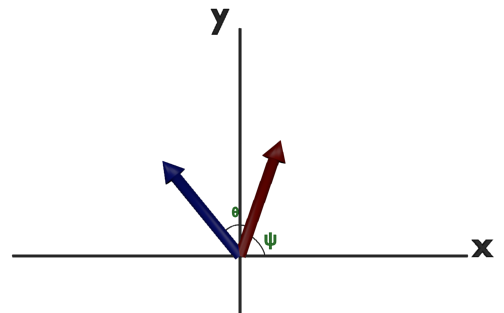
\includegraphics[height=0.4\textheight]{rotateVector}
    \vfill
    \column{0.65\textwidth}
    \dotfield{50}{24}
  \end{columns}
\end{frame}

\begin{frame}{Rotation Matrix In 2D (The Less Hard Way)}

  \begin{columns}
    \column{0.35\textwidth}
    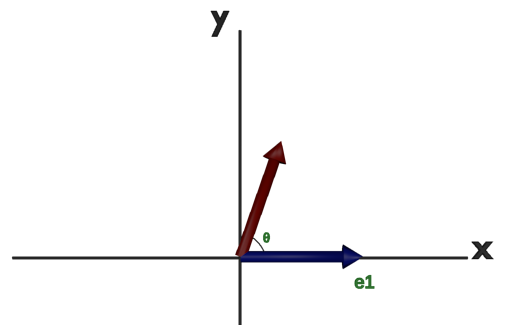
\includegraphics[height=0.4\textheight]{rotateVectorBasis}
    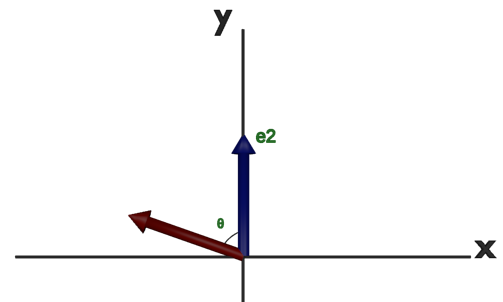
\includegraphics[height=0.4\textheight]{rotateVectorBasisE2}
    \column{0.65\textwidth}
    \dotfield{50}{24}
  \end{columns}
\end{frame}

\begin{frame}{The Identity Matrix}

  Suppose that $I_n\left(\vec{x}\right)=\vec{x}$. What is the standard
  matrix associated with it?

  \dotfield{60}{24}
  
\end{frame}


\begin{frame}{Blank Page}
  \dotfield{60}{24}
\end{frame}


\end{document}
